\documentclass[a4paper,11pt,dvipdfmx]{ujarticle}
% パッケージ
\usepackage{graphicx}
\usepackage{url}
% レイアウト指定を記述したファイルの読み込み
\input{layout}

% タイトルと氏名を変更せよ．
\title{日本におけるデジタル化の状況}
\author{G684182026 黄 鴻宣}

\begin{document}

\maketitle %ここにタイトルが入る
\section{デジタル競争力ランキング}

国際経営管理開発研究所（IMD）の調査\cite{imd}によると，日本のデジタル競争力ランキングは図\ref{fig51}に示すように，調査対象の64か国中総合で28位，準備分野で27位となっている．

\begin{figure}[htbp]
    \centering
    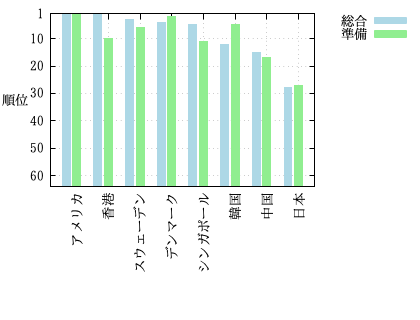
\includegraphics[width=0.7\linewidth]{fig51.png}
    \caption{デジタル競争力ランキング（64カ国中）}\label{fig51}
\end{figure}

\section{ブロードバンドの整備状況}

OECDによるプロードバンド回線の普及に関する調査\cite{oecd}によると、表\ref{tbl:加入者数}に示すように、日本におけ
る100人あたりの光ファイバー回線の加入者数は29.0で、韓国、スウェーデン、ノルウェーに続いて第
4位になっている.

\begin{table}[htbp]
    \centering
    \caption{光ファイバー回線の加入者数（100人あたり）}
    \label{tbl:加入者数}

    \begin{tabular}{|c|c|c|}
        \hline
        順位 & 国名&加入者数 \\
        \hline
        1位 & 韓国 & 38.2 \\
        \hline
        2位 & スウェーデン & 31.9 \\
        \hline
        3位     & ノルウェー & 29.5 \\
        \hline
        4位 & 日本 & 29.0 \\
        \hline
        5位 & アイスランド  &28.8\\
        \hline
        6位 & スベイン &27.3 \\
        \hline
        7位 &   ポルトガル &25.1\\
        \hline 
        8位 & ニュージーランド&23.6 \\
        \hline
        9位 & リトアニア&22.3 \\
        \hline
        10位 & フランス&21.2 \\
        \hline
    \end{tabular}
\end{table}

\section{考察}

データが示す通り、日本の光ファイバー普及率は世界4位と非常に高い。しかしその一方で、デジタル競争力ランキングでは64カ国中28位と、下位に低迷している。本調査の結果から、日本はネット環境は世界トップクラスに整っているが、それを十分に活かしきれていないと考えられる。

% ここから本文
% 節見出し: \section{}
% を使う

% 本文(1)
%  参考文献の参照: \cite{}
%  図番号の参照： \ref{}
% を使う
% 文献データベースのキーワードは oecd と imd
% になっている．

% 図の挿入
% \includegraphics{}
% を
% \begin{figure}[htbp]
% \end{figure}
% で囲み
% \caption{}
% で図のタイトルを入れる．
% \label{}
% を使って図番号が参照できるようにする
% また，
% \centering
% で図が中央に来るようにする

% ーーー
% 節見出し(2)

% 本文(2)

% 表の挿入
% \begin{tabular}
% \end{tabular}    
% による表の記述を 
% \begin{table}[htbp]
% \end{table}
% で囲み
% \caption{}
% で表のタイトルを入れる．
% \label{}
% を使って表番号が参照できるようにする
% また，
% \centering
% で表が中央に来るようにする

% ーーー
% 見出し(3)
% 考察
%
% \begin{itemize}
% \end{itemize}
% を使って箇条書きで記述する

% ここに参考文献が入る
%
\bibliographystyle{junsrt}
\bibliography{exercise.bib}

\end{document}